\section{Simulation Analysis}
\label{sec:simulation}

\subsection{Audio Amplifier Simulation}
\label{subsec:amp_simulation}
\par In this section we simulate an audio amplifier through the NGspice tool. Our goal is to simulate the audio amplifier using two different kinds of transistors (NPN and PNP). It is our objetive to measure the output voltage gain in the passband and the lower and upper 3dB cut off frequencies, as well as the input and output impedances.

\par  \textbf{Important note:} Beyond modelling and analysing the circuit provided, one of the goals of this laboratory assignment is to maximize the merit, which is computed according to the following formula:
\begin{equation}
M = \frac{\text{voltageGain}*\text{bandwidth}}{\text{cost}*\text{lowerCutoffFreq}}
\end{equation}

Therefore, it was our intention to obtain the best value for this parameter,using each of the variables in order to maximize it, wich means that we have not tried to improve each of those separately, but as a all.
In order to do it we used the values indicated in the begginig of Section \ref{sec:analysis} which resulted in the merit value bellow:

\begin{table}[H]
  \centering
  \begin{tabular}{ | m{11cm} | m{3cm}| } 
    \hline    
    {\bf Merit} & {\bf Value} \\ \hline
    Merit & 1.75991E-10\\ \hline
Cost & 673324 MU\\ \hline

  \end{tabular}
  \caption{Merit Calculation}
  \label{tab:merit}
\end{table}

\subsection{Output Voltage Gain}
\label{output_gain}
\par In order to measure the output voltage gain, we used Ngspice's \textit{measure} function to determine the maximum value of the output voltage. By definition the gain is the magnitude coefficient between the output voltage and the input voltage. In this particular case, the input voltage has a magnitude of 1V, wich means that we can reduce the calculation of the gain phase and magnitude to the output voltage.

 In the following table, we present the maximum magnitude of the gain (v(out)), in decibels:
 
\begin{table}[H]
  \centering
  \begin{tabular}{|l|r|}
    \hline    
    {\bf Output Voltage Gain} & {\bf Value} \\ \hline
    Output Voltage Gain dB & 266.369\\ \hline
Central Freq & 949.276\\ \hline
Low CO Freq & 453.95\\ \hline
Up CO Freq & 1985.08\\ \hline
Gain Deviation & 166.369\\ \hline
Gain Deviation dB & 8.50966\\ \hline
Central Freq Deviation &50.724\\ \hline
Bandwidth & 1531.13\\ \hline

  \end{tabular}
  \caption{Maximum Gain Magnitude, in dB}
  \label{tab:gain}
\end{table}



\subsection{Frequency response}
\label{frequency_response}
In this subsection, the same function as in the subsection \ref{output_gain} (\textit{measure}) was used to compute the value of the lower and upper 3db cut off frequencies, which allowed the calculation of the bandwidth, which is the difference of the two variables previosuly mentioned. The results obtained are shown in the table bellow:

\begin{table}[H]
  \centering
  \begin{tabular}{|l|r|}
    \hline    
    {\bf Variable} & {\bf Value [Hz]} \\ \hline
    low & 8.880418e+03\\ \hline
up & 1.603742e+06\\ \hline
bandwidth & 1.594862e+06\\ \hline

  \end{tabular}
  \caption{Lower and Upper Cut off Frequencies and Bandwidth, in Hz}
  \label{tab:frequency_response}
\end{table}


In order to compare and understand the evolution of the circuit from the gain stage to the output stage we firtly show the magnitude and the the phase plots in the collector node (the output of the gain stage) and then the same quantities regarding the output stage:

\begin{figure}[H] \centering
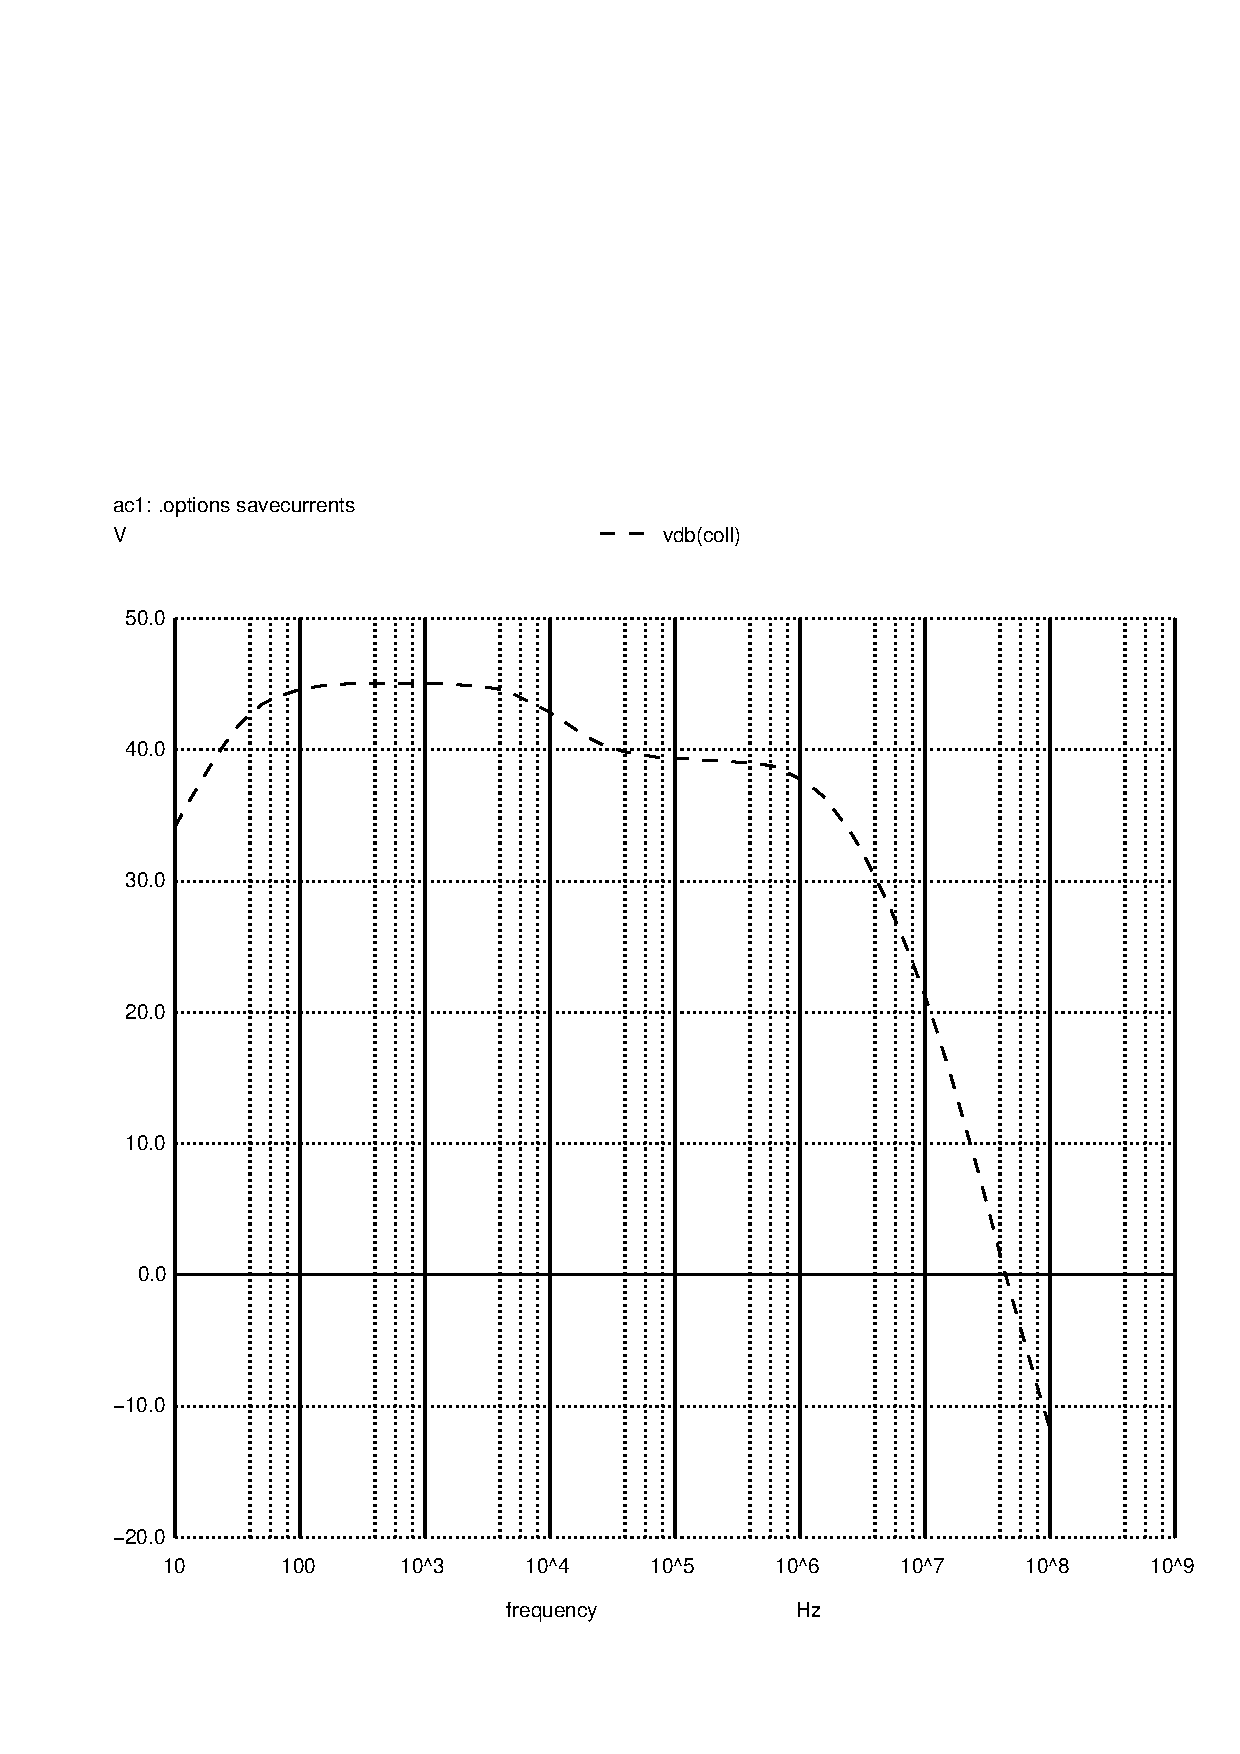
\includegraphics[clip, trim=1.3cm 1.3cm 0cm 7cm, width=0.6\linewidth]{vcolldb.pdf}
\caption{v(coll) magnitude, in dB}
\label{fig:voutdb}
\end{figure}

\begin{figure}[H] \centering
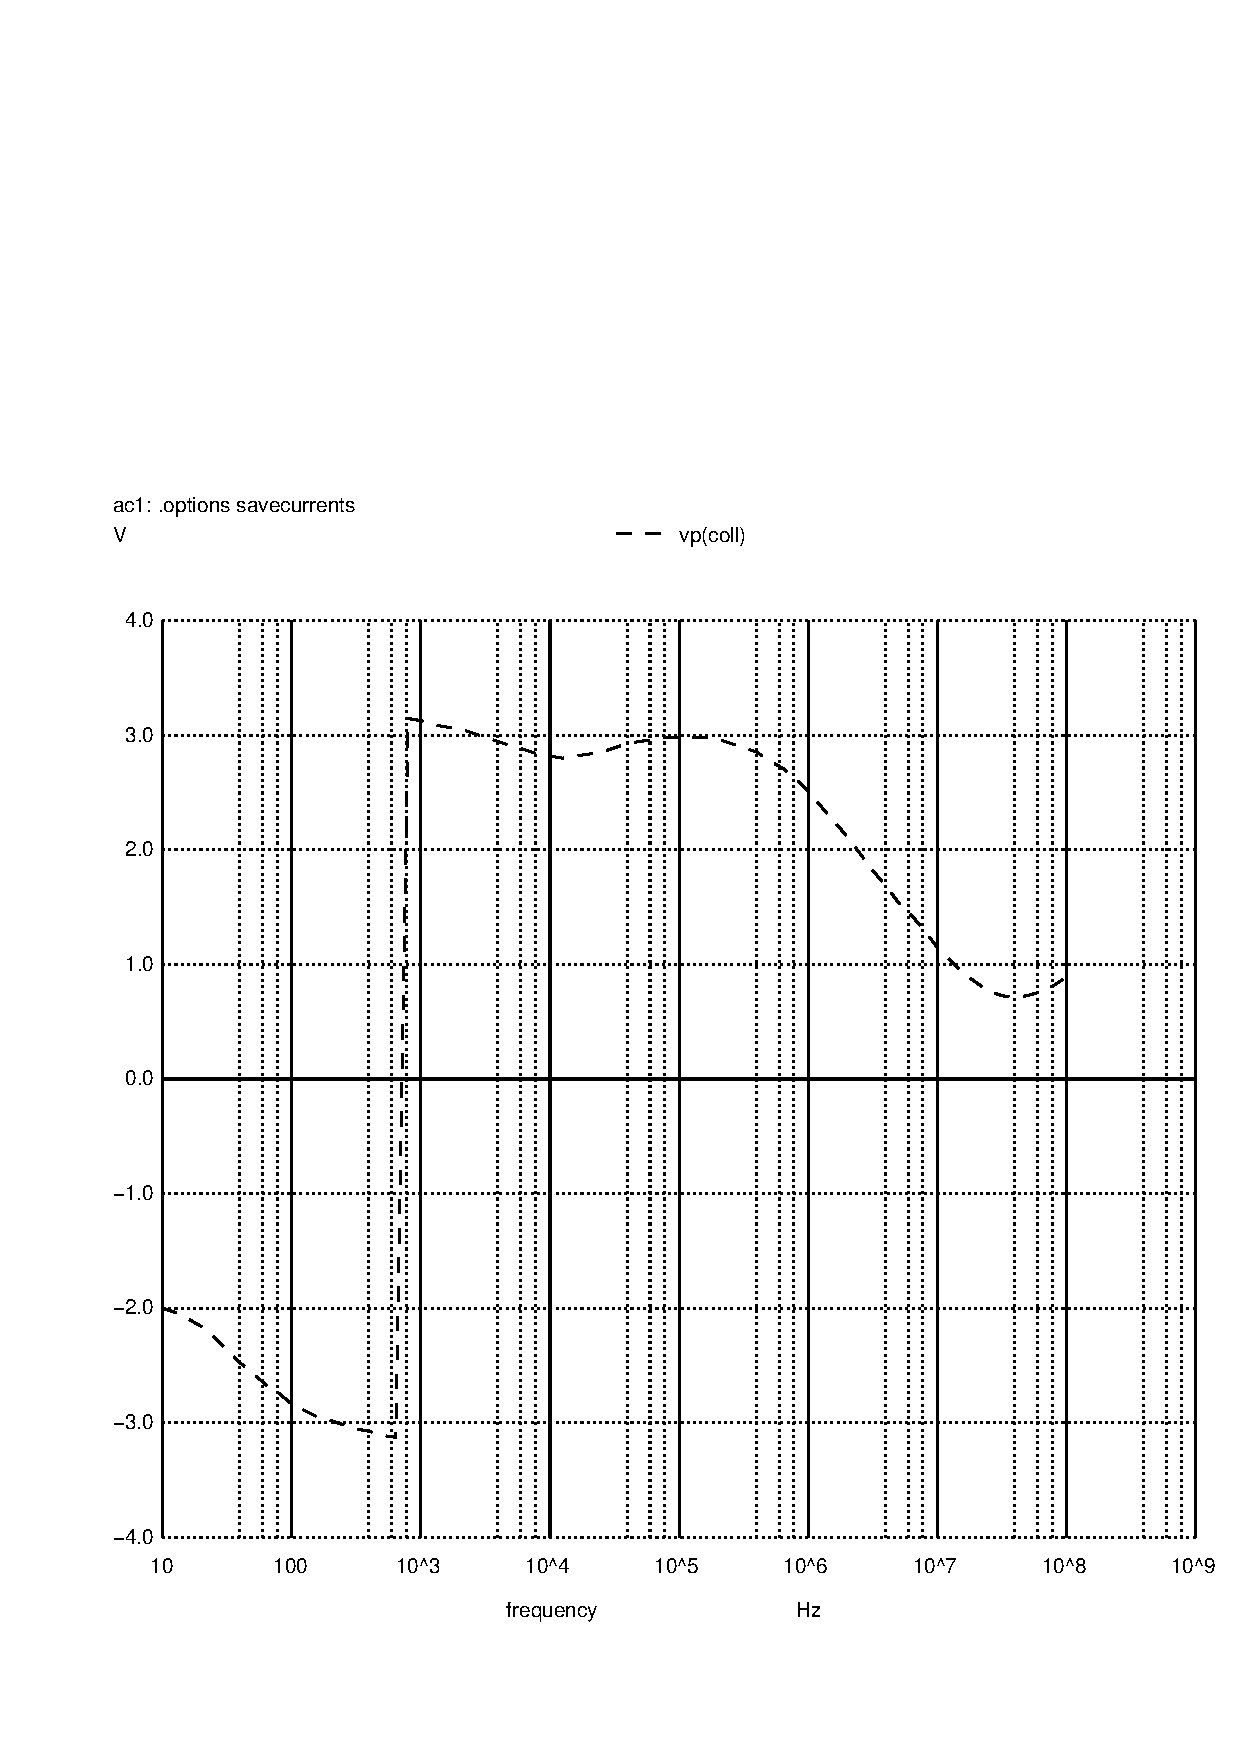
\includegraphics[clip, trim=1.3cm 1.3cm 0cm 7cm, width=0.6\linewidth]{vcollp.pdf}
\caption{v(coll) phase, in rad}
\label{fig:voutp}
\end{figure}


 Next, we present the graphical representation of both the magnitude and the phase frequency response at the output stage:
 

\begin{figure}[H] \centering
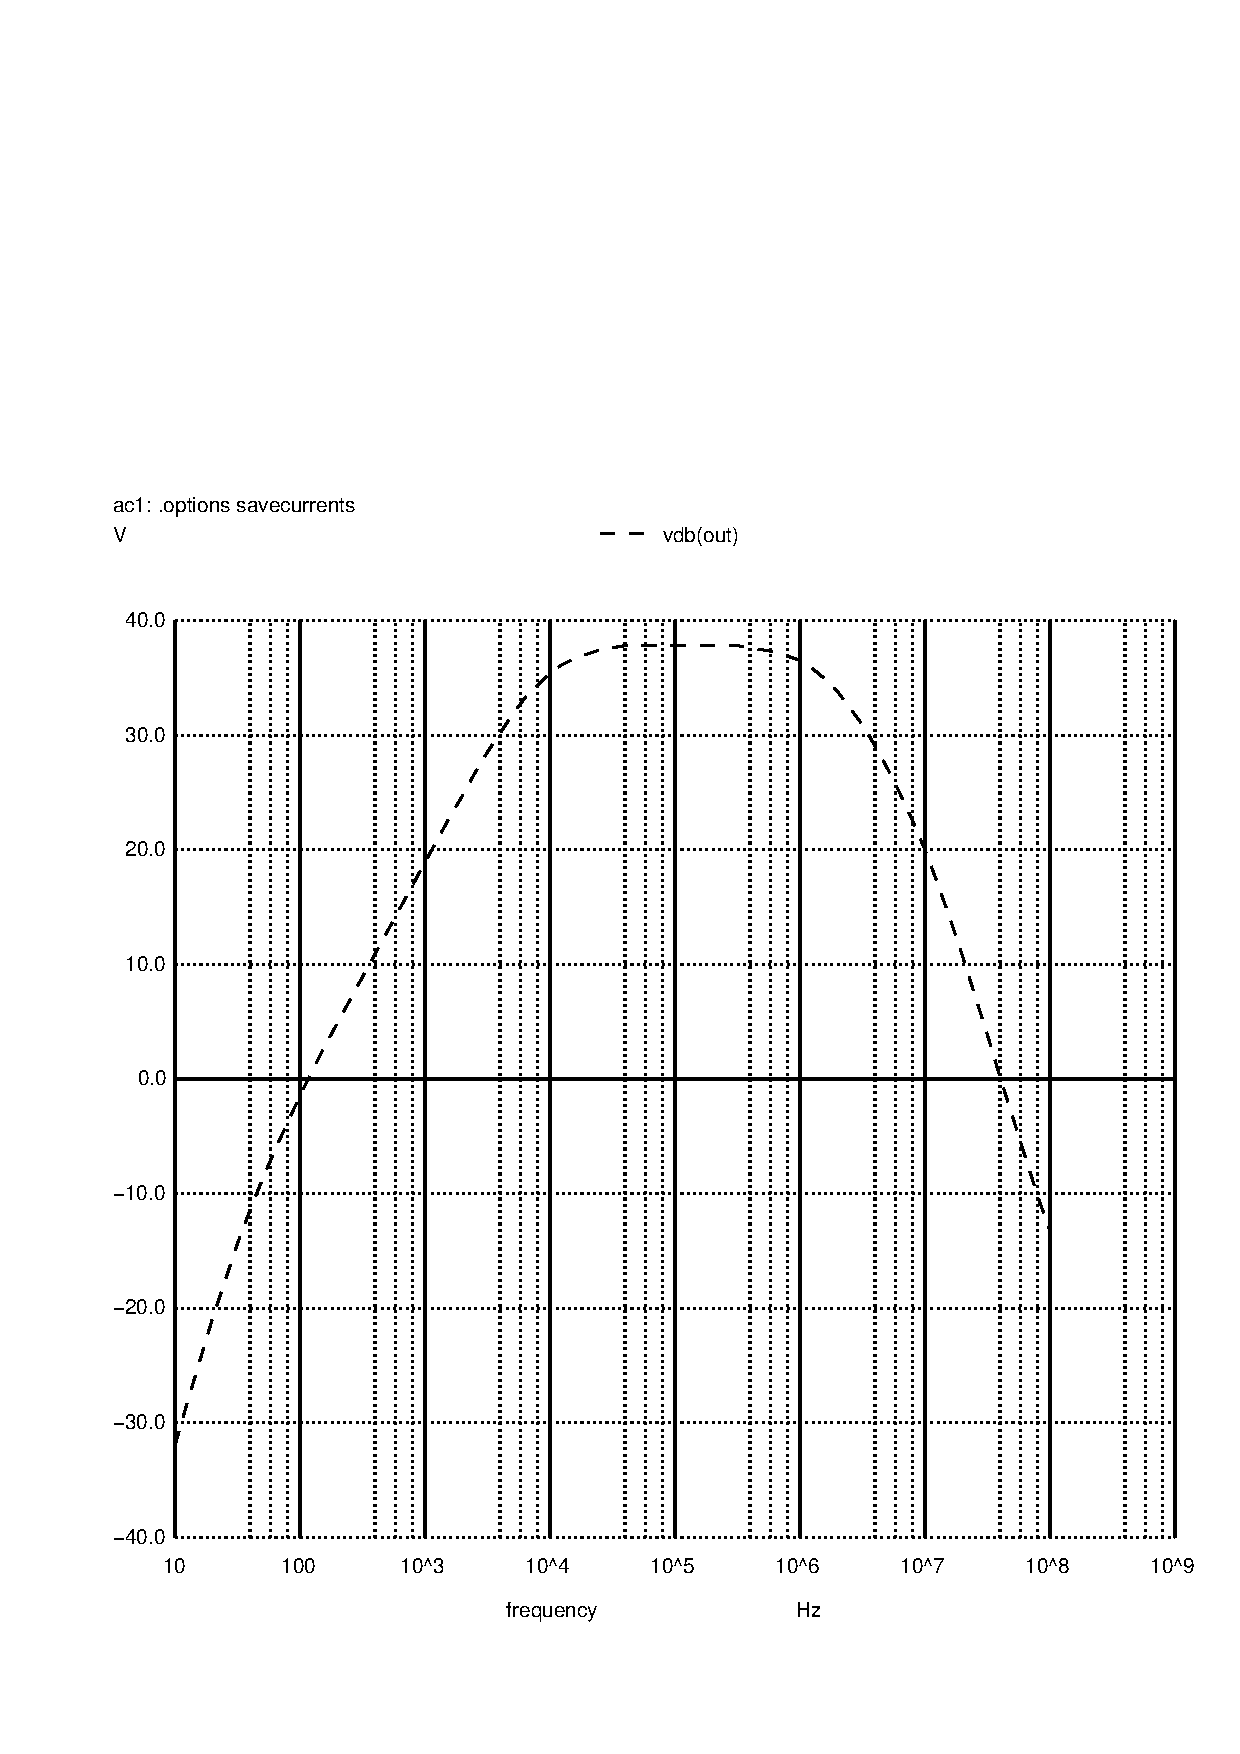
\includegraphics[clip, trim=1.3cm 1.3cm 0cm 7cm, width=0.6\linewidth]{voutdb.pdf}
\caption{Gain / v(out) magnitude, in dB}
\label{fig:voutdb}
\end{figure}

\begin{figure}[H] \centering
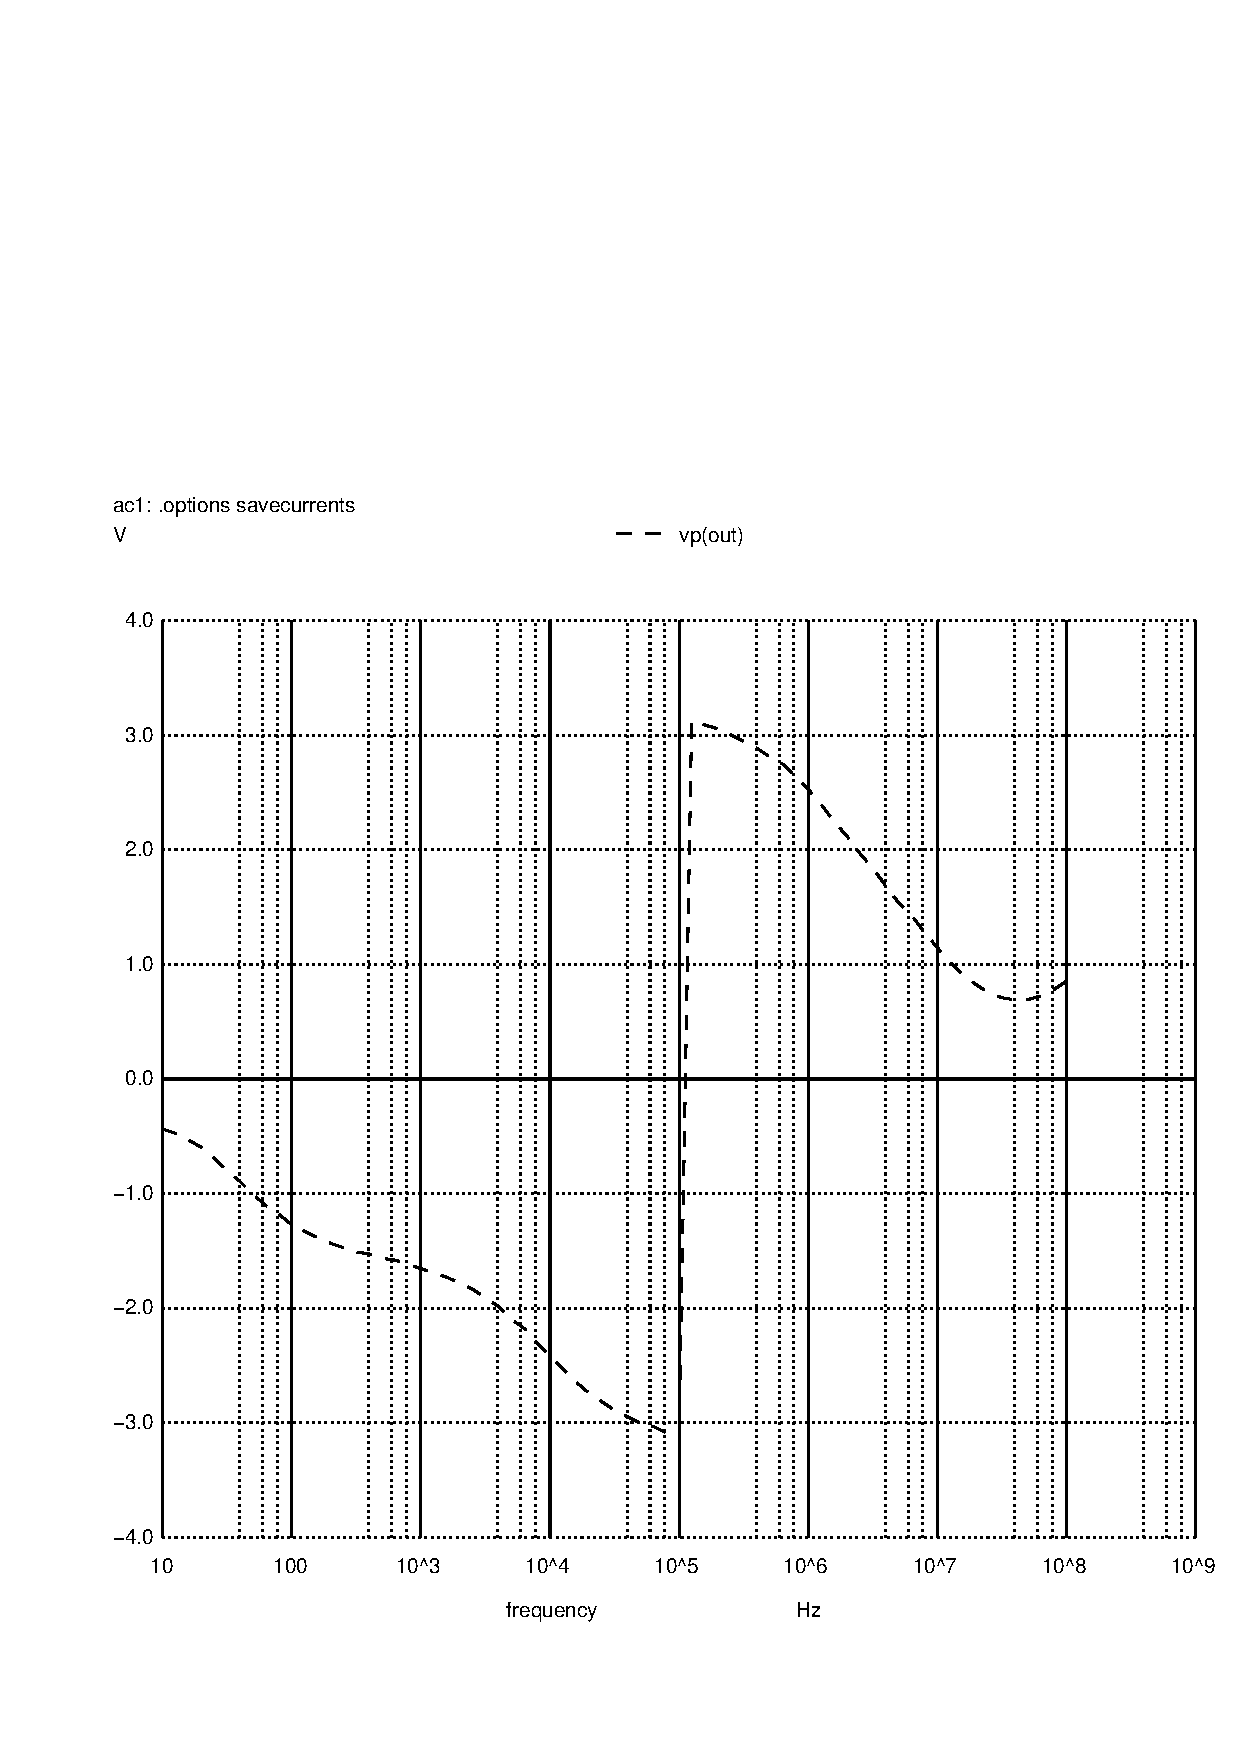
\includegraphics[clip, trim=1.3cm 1.3cm 0cm 7cm, width=0.6\linewidth]{voutp.pdf}
\caption{Gain / v(out) phase, in rad}
\label{fig:voutp}
\end{figure}


\subsection{Input impedances}
Finally, in this subsection the input impedance and the output impedance are presented. We can verify from them values that we achieved the goal of having a high input impedance and a low output impedance, wich allow to obtain a better amplifier:


\begin{table}[H]
  \centering
  \begin{tabular}{|l|r|}
    \hline    
    {\bf Input Impedance} & {\bf Value [S]} \\ \hline
    zi & 5.638527e-01,-8.44302e-02\\ \hline

  \end{tabular}
  \caption{Input Impedance, in Siemens}
  \label{tab:input_z}
\end{table}


\begin{table}[H]
  \centering
  \begin{tabular}{|l|r|}
    \hline    
    {\bf Output Impedance} & {\bf Value [S]} \\ \hline
    zo & -1.00554e+01,1.184265e+00\\ \hline

  \end{tabular}
  \caption{Output Impedance, in Siemens}
  \label{tab:output_z}
\end{table}



